\documentclass[12pt, titlepage]{article}

\usepackage{booktabs}
\usepackage{tabularx}
\usepackage{hyperref}
\hypersetup{
colorlinks,
citecolor=black,
filecolor=black,
linkcolor=red,
urlcolor=blue
}
\usepackage[round]{natbib}
\usepackage{graphicx}
%% Comments

\usepackage{color}

\newif\ifcomments\commentstrue

\ifcomments
\newcommand{\authornote}[3]{\textcolor{#1}{[#3 ---#2]}}
\newcommand{\todo}[1]{\textcolor{red}{[TODO: #1]}}
\else
\newcommand{\authornote}[3]{}
\newcommand{\todo}[1]{}
\fi

\newcommand{\wss}[1]{\authornote{blue}{SS}{#1}}
\newcommand{\an}[1]{\authornote{magenta}{Author}{#1}}


\begin{document}

\title{Stock Prediction System} 
\author{Renjie Zhang}
\date{\today}
\maketitle

\pagenumbering{roman}

\section{Revision History}

\begin{tabularx}{\textwidth}{p{3cm}p{2cm}X}
\toprule {\bf Date} & {\bf Version} & {\bf Notes}\\
\midrule
2017-10-06 & 1.0 & create\\
2017-10-09 & 1.1 & update\\
\bottomrule
\end{tabularx}

~\newpage

\section{Symbols, Abbreviations and Acronyms}

\renewcommand{\arraystretch}{1.2}
\begin{tabular}{l l} 
\toprule 
\textbf{symbol} & \textbf{description}\\
\midrule 
T & Test\\
SVM & Support Vector Machine\\
RDD &Resilient Distributed Datasets\\
K & Kernel function\\
X & features of the data (date , price)\\
C& The price from different days\\
$\beta$ & The error modifier\\
y& The result between 1 and -1\\ 
\bottomrule
\end{tabular}\\



\newpage

\tableofcontents

\listoftables

\listoffigures

\newpage

\pagenumbering{arabic}



\section{General Information}
This Document is a test plan of the software-Stock Prediction System which is a tool used to predict the stock prices using machine learning. The software will be worked on a distributed system.

\subsection{Purpose}

This test plan describes the testing methods that will drive the testing of the
Stock Prediction System and give a guide to the users about the QA. This
document includes the descriptions of testing tool, testing functions, unit
testing method and system test. Based on these testing, the users may cache the
functional and non functional issues from the first release of the software and
find out the improvement.

\subsection{Scope}

The testing plan will cover both system testing and unit testing. This software is wrote by Python. The functions
are the data input, data format validation, calculation of SVM, data plot, Spark
RDD Distributed System, and the output of the result. Basically every part of
the system will be tested, and most of the testing will be done by unit testing.
For more information please read the SRS in my repository: 
\url{https://github.com/renjiezhang/CAS-741}.\\


\subsection{Overview of Document}
This document explains the testing plan for the software - Stock Prediction
System. It includes the briefcase of software description, the different testing
methods - unit testing and integration testing, testing tools. It will cover
both functional and non functional requirements.
\section{Plan}
In this section, the general description of the testing plan for the software and corresponding testing tools will be introduced.
\subsection{Software Description}
The Stock Prediction System is used to analyze the future trend of stocks. The prediction was provided by machine learning algorithms based on the historical data. 
The system will be run on a big data platform (Spark), to obtain the more accurate results. In this case, we need to setup a distributed system to support Spark.
\subsection{Test Team}

Renjie Zhang

\subsection{Automated Testing Approach}
NA
\subsection{Verification Tools}
Python unit testing : This framework was included in Python standard library. It is easy to use by people familiar with the xUnit frameworks, strong support for test organization and reuse via test suites\\
Wing : A popular Python IDE which contents the code checking and indent correction.\\

% \subsection{Testing Schedule}
% See Gantt Chart at the following url ...

\subsection{Non-Testing Based Verification}
NA

\section{System Test Description}
This section describes the testing on the system environment, such as the data file input and spark distribution system. Users need to make sure the application run on the system without any issues. 
\subsection{Tests for Functional Requirements}
The functional requirements includes the data input, the data format verification, the Spark RDD transaction, the plot generation and the display of the output. The software must fulfill all of the functional requirements without issues.

\subsubsection{Data Input}
The system needs to load a dataset from a CSV file. This test ensures the data input method. 
\paragraph{File loading Testing }

\begin{enumerate}

\item{File is loaded successfully\\}

Type: Functional, Manual, Static etc.
Initial State: NA
Input: File Path
Output: Successful Message
How test will be performed: System tries to load the data set file based on the file name and location without issues.

\item{Input Data Validation\\}

Type: Functional, Manual\\
Initial State: NA\\
Input: Data from the file\\
Output: A successful message.\\
How test will be performed: System have to ensure the data type and format is
correct for each columns of the file : the pattern of the date, the formats
of the price and number of digits of decimals. If the format does match the requirement, the program will encounter an IO exception.
The example of the CSV file is shown in the following figure. 

~\newline
\begin{figure}[h!]
\begin{center}
%\rotatebox{-90}
{
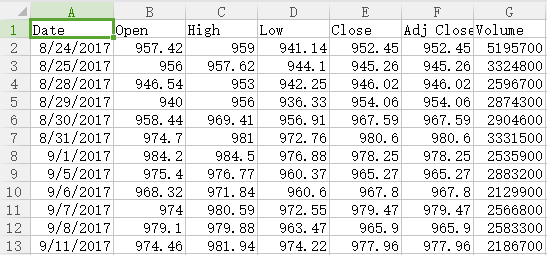
\includegraphics[width=0.5\textwidth]{amazon.png}
}
\caption{\label{Input Data}}
\end{center}
\end{figure}

~\newline
\item{Plot Testing\\}

Type: Functional, Manual, Static
Initial State: NA\\
Input: A pre-defined Array\\
Output: A correct plot\\
How test will be performed: System reads the data and generate a plot using the price and the date as the x and y axis.\\

\end{enumerate}

\subsubsection{Distributed System}
This section focus on the distributed system of Spark platform. It guides the
users to test the data flow on the spark system. RDD is the format of data flow
in Spark. testers need to double check the data was distributed into each
workers through RDD.

\paragraph{ Spark RDD Testing}

\begin{enumerate}

\item{Data is distributed to workers\\}

Type: Functional, Manual, Static\\
Initial State: NA\\
Input:There will be a list of numbers to input to the RDD function. To test the RDD function, the driver will ask Spark to return some random number back. \\
Output: The list of numbers which is collected back from workers.\\
How test will be performed: There will be an input array to the driver, driver assign the array to each workers. Each worker receives part of the numbers in the list. When the driver collect the RDD, works return each part of the number back to driver. A sample work flow is shown below:
~\newline
\begin{figure}[h!]
\begin{center}
%\rotatebox{-90}
{
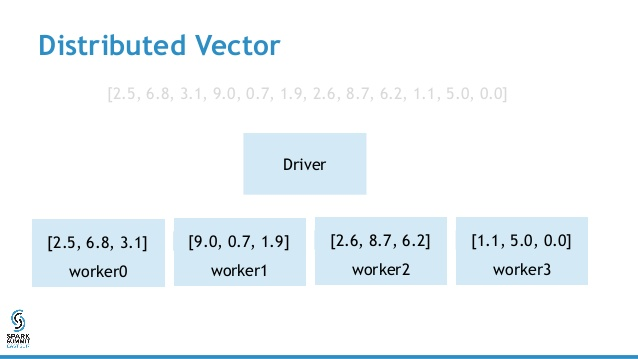
\includegraphics[width=0.5\textwidth]{sparkrdd.png}
}
\caption{\label{Input Data}}
\end{center}
\end{figure}

\end{enumerate}

\subsection{Tests for Non functional Requirements}
Non functional requirements are not as prior as functional requirements, but it is still necessary to have tests on them in order to improve the software performance and quality.
\subsubsection{Big Data System Testing}
In this section, the only requirement is the performance.
\paragraph{ Performance Testing}

\begin{enumerate}

\item{Performance of the workers\\}

Type: Manual
Initial State: NA
Input/Condition: NA
Output/Result: Result of the time cost\\
How test will be performed: \\
Chang the size of the dataset files by downloading the files with different date range. For example, reduce the date range from 5 years to 3 years and compare the performance. \\
Change the number of date parameter to predict short term and long term stock price. By adding a new type of number of date, the software need to increase the run time. \\


\end{enumerate}

\newpage
\subsection{Traceability Between Test Cases and Requirements}

\begin{table}[h!]
\centering
\begin{tabular}{|c|c|c|c|c|c|c|c|}
\hline
& Input & Plot & Data Validation & Calculation & Output& Performance\\
\hline
Input Data &X & & & & \\ \hline
Data Validation &X & &X & & &X \\ \hline
RDD &X & & & & & & \\ \hline
Plot & &X & & & &X \\ \hline
Kernelling & & & & X& &X \\ \hline
Volatility & & & &X & & \\ \hline 
Momentum & & & &X & & \\ \hline 
Prediction & & & &X &X & \\ \hline 


\end{tabular}
\caption{Traceability Matrix Showing the Connections Between Requirements and Test Cases}
\label{Table:R_trace}
\end{table}

% \section{Tests for Proof of Concept}

% \subsection{Area of Testing1}
% \paragraph{Title for Test}

% \begin{enumerate}

% \item{test-id1\\}

% Type: Functional, Dynamic, Manual, Static etc.
% Initial State: 
% Input: 
% Output: 
% How test will be performed: 
% \item{test-id2\\}

% Type: Functional, Dynamic, Manual, Static etc.
% Initial State: 
% Input: 
% Output: 
% How test will be performed: 

% \end{enumerate}

% \subsection{Area of Testing2}

% ...
\section{Unit Testing Plan}
The unit testing plan will involve the following modules: Load Data, SVM Kernelling, Volatility Calculating, Momentum Calculating, Predict and Output.\\
\begin{enumerate}

\item{ Calculate Volatility\\}
This function is use to calculate the price volatility and index volatility. Since the calculation is similar they share the same function. A correct result is expected by inputting the parameters to the equation \\
$\frac{\sum_{i=t-n+1}^{t} \frac{C_i-C_{i-1}}{C{i-1}}}{n}$ \\ 

Input: A pre-defined Array of stock record, which contains two elements: price and date\\
Output: An array of price volatility based on the input array\\


\item{ Calculate Momentum\\}
This function is use to calculate the price momentum and index momentum. Since the calculation is similar they share the same function. A correct result is expected by inputting the parameters to the equation \\
$\frac{\sum_{i=t-n+1}^{t} \frac{C_i-C_{i-1}}{C{i-1}}}{n}$ \\ 

Input: A pre-defined Array of stock record, which contains two elements: price and date\\
Output: An array of price volatility based on the input array\\


\item{Predict \\}
The Predict module receives a set of parameters calculated from the previous functions and returns a result. A correct result is expected by inputing the parameters to the equation \\\\
$y=\beta _0+\sum {a_iy_iK(x(i),x)}$\\
Input: Two pre-defined lists of stock record, which contains two elements: price and date. They have same format, one is for stock price and another is for NASDQ Index record\\
Output:A score of a decimal number which represents the probability\\

\end{enumerate} 

\bibliographystyle{plainnat}

\bibliography{SRS}

\newpage

\section{Appendix}

NA

\subsection{Symbolic Parameters}

NA

\subsection{Usability Survey Questions?}

NA

\end{document}


